\documentclass[12pt]{article}

%% preamble: Keep it clean; only include those you need
\usepackage{amsmath}
\usepackage[margin = 1in]{geometry}
\usepackage{graphicx}
\usepackage{booktabs}
\usepackage{natbib}
\usepackage{setspace}
\usepackage{listings}

% for space filling
\usepackage{lipsum}
% highlighting hyper links
\usepackage[colorlinks=true, citecolor=blue]{hyperref}


%% meta data

\title{Electronic Sports: Winner Prediction}
\author{Hao Ding\\
  Department of Statistics\\
  University of Connecticut
}



\begin{document}
\maketitle

\doublespacing

\begin{abstract}
	
This paper explores factors influencing player success in the popular online multiplayer battle royale game, PlayerUnknown's Battlegrounds (PUBG). Utilizing data from the PUBG Developer API, which includes information from over 65,000 recorded games, we employ correlation analysis, feature importance from tree-based models, and recursive feature elimination to identify key elements impacting player performance. The dataset encompasses various metrics such as assists, boosts, revives, damage dealt, team kills, kill place, distance traveled, weapons acquired, match duration, and win place percentile. Our analysis reveals correlations between different factors and highlights the significance of kills and walk distance in achieving better win placements. The methods section details the approach, including the use of ensemble models like Random Forest and Gradient Boosting, as well as deep learning models for predictive tasks. The discussion emphasizes the need for a large and diverse dataset, periodic model updates due to game dynamics, collaboration with PUBG experts, and the inherent unpredictability of player strategies. While machine learning models offer valuable insights, they should be interpreted cautiously, recognizing the game's dynamic nature and unpredictable elements.  

\end{abstract}


\section{Introduction}
\label{sec:intro}

PUBG (PlayerUnknown's Battlegrounds) represents a pivotal development in the gaming world, particularly within the rapidly growing eSports sector. This game, a brainchild of PUBG Corporation, a subsidiary of the South Korean company Bluehole, has not only garnered immense popularity but also significantly influenced the battle royale genre since its inception in March 2017. Its design, inspired by the Japanese film "Battle Royale", offers a unique blend of survival, exploration, and combat, making it a standout in the gaming community.

The gameplay of PUBG is both engaging and complex. It drops up to 100 players onto an island where they must scavenge for weapons and equipment. The players then battle it out, with the play area gradually shrinking, forcing closer encounters and intensifying the game's pace. This innovative approach has not only attracted millions of players worldwide but also set new precedents for interactive and competitive gaming. As a result, PUBG has been a driving force behind the explosion of the battle royale genre, influencing numerous other games and becoming a staple in competitive gaming events like the PUBG Global Championship.

In recent years, the intersection of data analytics and gaming has opened up new frontiers in understanding player behavior and game strategies. In competitive games like PUBG, where player decision-making and strategy are key, analyzing in-game data can yield insights into effective tactics, player tendencies, and overall game dynamics. This application of analytics is becoming increasingly crucial in the professional eSports arena, where understanding the nuances of player actions can give teams a competitive edge.

Our research focuses on leveraging this intersection of gaming and data analytics. By examining a comprehensive dataset from over 65,000 PUBG games, we aim to uncover the underlying factors that contribute to player success. Specifically, we are interested in identifying which behaviors and strategies lead to more kills or longer survival in the game, ultimately contributing to a player's or team's victory. This analysis not only has implications for player performance enhancement but also provides deeper insights into the strategic fabric of PUBG. Through this study, we hope to contribute to the growing body of knowledge in eSports analytics, offering both theoretical and practical insights into one of the most popular games in the modern gaming era.





% roadmap
The rest of the paper is organized as follows.
The data will be presented in Section~\ref{sec:data}.
The methods are described in Section~\ref{sec:meth}.
The results are reported in Section~\ref{sec:resu}.
A discussion concludes in Section~\ref{sec:disc}.


\section{Data}
\label{sec:data}



Our dataset was sourced from the PUBG Finish Placement Prediction competition on Kaggle. This dataset includes a wide range of variables collected from actual PUBG games, offering a rich foundation for analyzing player behavior and game outcomes.

\subsection{Sample Size and Representation}

The dataset comprises data from over 65,000 PUBG matches, encompassing a diverse array of player skills and strategies. This extensive collection allows for a detailed examination of various factors influencing player success in PUBG. we can see in the table \ref{table:variables}

\begin{table}[h!]
	\centering
	\begin{tabular}{|l|p{10cm}|}
		\hline
		\textbf{Variable} & \textbf{Description} \\
		\hline
		Assists & Number of enemy players this player damaged that were killed by teammates. \\
		\hline
		Boosts & Number of boost items used. \\
		\hline
		Revives & Number of times this player revived teammates. \\
		\hline
		Heals & Number of healing items used. \\
		\hline
		Damage Dealt & Total damage dealt. Self inflicted damage is subtracted. \\
		\hline
		TeamKills & Number of times this player killed a teammate. \\
		\hline
		Kill Place & Ranking in match of number of enemy players killed. \\
		\hline
		Kills & Number of enemy players killed. \\
		\hline
		Ride Distance & Total distance traveled in vehicles measured in meters. \\
		\hline
		Swim Distance & Total distance traveled by swimming measured in meters. \\
		\hline
		Walk Distance & Total distance traveled on foot measured in meters. \\
		\hline
		Weapons Acquired & Number of weapons picked up. \\
		\hline
		Match Duration & Duration of match in seconds. \\
		\hline
		Win Place Perc & Percentile winning placement, where 1 corresponds to 1st place, and 0 to last place. \\
		\hline
	\end{tabular}
	\caption{Description of Variables in the PUBG Dataset}
	\label{table:variables}
\end{table}


\subsection{Data Processing}

The data preprocessing was performed using R, employing a series of steps to ensure the integrity and suitability of the data for subsequent analysis. Initially, missing values within nominal predictors were handled by introducing a new level to represent novel categories, thus accounting for potential new factor levels that were not present during the training phase. For numeric predictors, missing values were imputed with the mean of the respective variables to preserve the dataset's integrity without introducing significant bias.

Furthermore, numeric predictors were standardized, scaling each feature to have a mean of zero and a standard deviation of one. This normalization is a crucial step, especially when employing algorithms that assume data is centered and scaled, such as support vector machines or k-means clustering.

The combined use of these preprocessing techniques ensures that the analysis is conducted on a dataset that is free from common issues that could undermine the validity of the results. Each step was carefully documented to maintain the reproducibility of the tudy.

\begin{lstlisting}[language=R, caption={R code for data preprocessing}, label={lst:datapreprocessing}]
	# Create the recipe
	rec <- recipe(~., data = data) %>%
	step_novel(all_nominal_predictors()) %>%
	step_unknown(all_nominal_predictors()) %>%
	step_impute_mean(all_numeric_predictors()) %>%
	step_normalize(all_numeric_predictors())
	
	# Prepare and bake the recipe
	prepped_data <- prep(rec, training = data)
	data_transformed <- bake(prepped_data, new_data = NULL)
\end{lstlisting}

\subsection{Statistical Summary}

A statistical summary is provided, showcasing the distribution and range of key variables such as damage dealt, distance traveled, and number of kills. This summary offers preliminary insights into general trends and patterns within PUBG gameplay.




\begin{table}[h!]
	
	\centering
	\begin{tabular}{|l|c|c|c|}
		\hline
		\textbf{Statistic} & \textbf{Damage Dealt} & \textbf{Ride Distance (meters)} & \textbf{Kills} \\ \hline
		Minimum            & 0.00                  & 0.00                           & 0.0000         \\ \hline
		1st Quartile       & 0.00                  & 0.00                           & 0.0000         \\ \hline
		Median             & 84.16                 & 0.00                           & 0.0000         \\ \hline
		Mean               & 129.74                & 590.99                         & 0.9184         \\ \hline
		3rd Quartile       & 185.40                & 0.01                           & 1.0000         \\ \hline
		Maximum            & 6229.00               & 40700.00                       & 58.0000        \\ \hline
	\end{tabular}
	\caption{Statistical Summary of Key Variables in PUBG Dataset}
	\label{table:stats_summary}
\end{table}

In this table \ref{table:stats_summary}, three key variables (Damage Dealt, Ride Distance, and Kills) from the PUBG dataset. It is observed that while most players have a lower number of kills (median of 0), some players achieve a significantly high number of kills (maximum of 58). Similarly, although most players travel short distances by vehicles, some cover distances as long as 40,700 meters. These figures reflect the diverse player behaviors in PUBG gameplay.






\section{Methods}

\subsection{Data Preprocessing}
Data preprocessing was a pivotal step in preparing the PUBG dataset for subsequent analysis. The process commenced with exploratory data analysis (EDA), which involved employing descriptive statistics and visualizations to unearth underlying trends, detect outliers, and observe patterns within the data. After EDA, we addressed missing values through appropriate imputation techniques, and feature engineering was undertaken to enhance the predictive capability of the dataset. This included encoding categorical variables and normalizing numerical variables to ensure uniformity.

A crucial part of preprocessing was the division of the dataset into training and testing sets. This split was essential for validating the model's performance and ensuring its ability to generalize to new, unseen data. Typically, a portion of the data (e.g., 70-80 percentage) was allocated to the training set, with the remainder reserved for testing.

Moreover, to refine the feature set and improve model efficiency, a correlation analysis was conducted. This analysis helped identify and eliminate highly correlated variables, thereby reducing dimensionality and potential multicollinearity issues. Variables with high correlation were evaluated, and those offering less informational value were selectively removed. This step was crucial to simplify the model, enhance interpretability, and potentially improve performance by focusing on the most relevant predictors.

In addition to the initial preprocessing steps, the data was further manipulated to facilitate a more straightforward interpretation of the results. Specifically, the continuous variable `winPlacePerc`, representing the percentile rank of a player's finish in a match, was transformed into a categorical factor with two levels: `defeat` and `win`. This dichotomy was established based on whether the player's rank was less than the top percentile (1), with the rationale that a victory can be considered as achieving the highest possible rank in a match. The code snippet below illustrates this transformation in R:

\begin{lstlisting}[language=R, caption=Creating a binary outcome variable]
	df3 <- df2 %>%
	mutate(win = factor(winPlacePerc < 1, c(TRUE, FALSE), 
	c("defeat", "win")))
\end{lstlisting}

This transformation was pivotal in simplifying the analysis, allowing subsequent models to predict a binary outcome of either winning or not winning, which is more aligned with common objectives in game outcome predictions.


\begin{figure}[h]
	\centering
	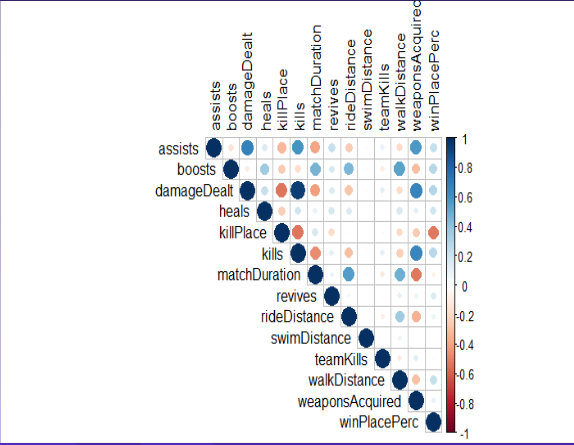
\includegraphics[width=0.75\textwidth]{Correlation.png} 
	\caption{Correlation matrix of PUBG gameplay variables.}
	\label{fig:correlation_matrix}
\end{figure}

Figure \ref{fig:correlation_matrix} presents the correlation matrix of selected gameplay variables from the PUBG dataset. Each cell in the matrix provides the correlation coefficient between two variables, ranging from -1 to 1. A positive correlation (closer to 1) suggests a direct relationship, where an increase in one variable tends to be associated with an increase in the other. Conversely, a negative correlation (closer to -1) indicates an inverse relationship. Notably, the variables such as `kills` and `winPlacePerc` show a strong positive correlation, implying that higher kills are strongly associated with better placement in a match.






\subsection{Model Selection}
Considering the project's aim to predict player success in PUBG, both regression and classification models were deemed suitable. Initial models included decision trees to establish a baseline performance. To capture more complex relationships within the data, advanced models such as Least Absolute Shrinkage and Selection Operator(Lasso Regression), Specified Lasso, and Support Vector Machines (SVM) were also employed. These models were chosen for their ability to handle large datasets and provide insights into feature importance.


\begin{figure}[h]
	\centering
	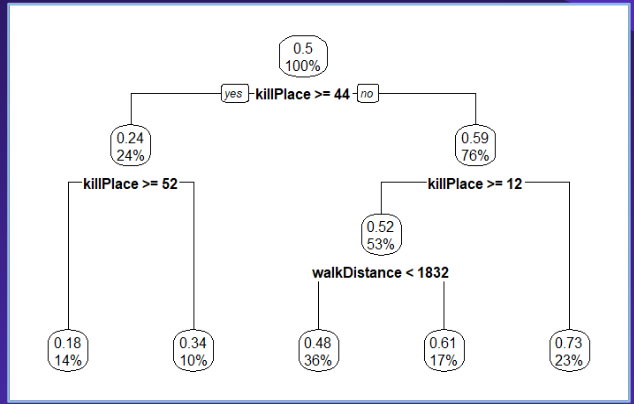
\includegraphics[width=\linewidth]{tree.png} 
	\caption{Decision tree model based on PUBG gameplay variables.}
	\label{fig:decision_tree}
\end{figure}

In our model training phase, we utilized a decision tree method, leveraging variables identified as significant from the correlation analysis. As illustrated in Figure \ref{fig:decision_tree}, the decision tree segregates players into groups based on `killPlace` and `walkDistance`. The tree structure indicates that `killPlace` is the most significant variable, initially splitting the players at a `killPlace` threshold of 44. Further splits are made based on additional thresholds of `killPlace` and `walkDistance`, highlighting their impact on the prediction of winning. Notably, `winPlacePerc` was not used as a predictor in this model. Instead, `win`, a binary outcome derived from `winPlacePerc`, was used to train the model, aligning with the objective to predict the likelihood of winning a match.


\section{Model Descriptions}

\subsection{Lasso Regression}
Lasso Regression, or Least Absolute Shrinkage and Selection Operator, is a type of linear regression that includes a penalty term to shrink coefficients towards zero. The objective function of Lasso Regression is given by:

\begin{equation}
	\min_{\beta} \left\{ \frac{1}{2n} \sum_{i=1}^{n} (y_i - \beta_0 - \sum_{j=1}^{p} \beta_j x_{ij})^2 + \lambda \sum_{j=1}^{p} |\beta_j| \right\}
\end{equation}

where $y_i$ is the response variable, $\beta_0$ is the intercept, $\beta_j$ are the coefficients, $x_{ij}$ are the predictor variables, $n$ is the number of observations, $p$ is the number of predictors, and $\lambda$ is the regularization parameter that controls the strength of the penalty. The Lasso penalty encourages sparsity in the coefficients, effectively performing variable selection by setting less important variable coefficients to zero.

\subsection{Specified Lasso}
The Specified Lasso is an extension of the Lasso Regression which allows for the inclusion of prior knowledge or structure in the model. It works on the principle that not all predictors are equal and enables the specification of groups among the predictors. The formulation of the Specified Lasso can be represented as:

\begin{equation}
	\min_{\beta} \left\{ \frac{1}{2n} \sum_{i=1}^{n} (y_i - \beta_0 - \sum_{j=1}^{p} \beta_j x_{ij})^2 + \lambda \sum_{k=1}^{K} w_k \sum_{j \in G_k} |\beta_j| \right\}
\end{equation}

where $G_k$ represents the groups of predictors, $w_k$ are weights that can be assigned to different groups reflecting their importance or confidence in the group's relevance to the response variable. This allows for differential shrinkage of coefficients and can incorporate domain knowledge into the model.

\subsection{Support Vector Machines (SVM)}
Support Vector Machines (SVM) are a set of supervised learning methods used for classification, regression, and outliers detection. The principle of SVM is to construct a hyperplane or set of hyperplanes in a high-dimensional space, which can be used for classification, regression, or other tasks. The optimal hyperplane is the one that represents the largest separation, or margin, between the two classes. In two-dimensional space, this hyperplane is a line dividing a plane into two parts where each class lays on either side.

For linear SVM, the objective is to find the hyperplane that has the maximum margin, which is formulated as:

\begin{equation}
	\min_{\mathbf{w}, b} \frac{1}{2} ||\mathbf{w}||^2 \quad \text{subject to} \quad y_i (\mathbf{w} \cdot \mathbf{x}_i + b) \geq 1, \, \forall i
\end{equation}

where $\mathbf{w}$ is the weight vector, $b$ is the bias term, $\mathbf{x}_i$ are the input features, and $y_i$ are the class labels.

For non-linear classification, SVM uses a kernel function to transform the input space into a higher-dimensional space where a linear separator can be used. The most common kernel functions include the linear, polynomial, radial basis function (RBF), and sigmoid kernels.

The dual form of the SVM optimization problem, which incorporates kernel functions, is given by:

\begin{equation}
	\max_{\alpha} \sum_{i=1}^{n} \alpha_i - \frac{1}{2} \sum_{i,j=1}^{n} y_i y_j \alpha_i \alpha_j k(\mathbf{x}_i, \mathbf{x}_j) \quad \text{subject to} \quad \sum_{i=1}^{n} y_i \alpha_i = 0 \quad \text{and} \quad 0 \leq \alpha_i \leq C, \, \forall i
\end{equation}

where $\alpha_i$ are the Lagrange multipliers, $k(\mathbf{x}_i, \mathbf{x}_j)$ is the kernel function, and $C$ is the penalty parameter of the error term.



\section{Model Training and Evaluation}

\subsection{Model Training}
Model training involves fitting the selected machine learning algorithms to the training data to learn the patterns that can predict the target variable. In this study, three models were trained: Lasso Regression, Specified Lasso, and Support Vector Machines (SVM).

For the Lasso and Specified Lasso models, a grid search was performed to find the optimal regularization parameter \(\lambda\) that minimizes the cross-validation error. This parameter controls the trade-off between simplicity (fewer variables) and fitting ability.

For the SVM model, both the kernel type and the regularization parameter \(C\) were optimized using cross-validation. The kernel transforms the data into a higher-dimensional space, while \(C\) controls the trade-off between maximizing the margin and minimizing the classification error.

\subsection{Model Evaluation}
The performance of each model was evaluated using a hold-out test set, which was not used during the training phase. The evaluation metrics included accuracy, precision, recall, and the F1 score for classification tasks, and the mean squared error (MSE) for regression tasks.

A confusion matrix was also constructed for each classification model to provide a clear breakdown of true positives, false positives, true negatives, and false negatives.

Additionally, Receiver Operating Characteristic (ROC) curves and Area Under the ROC Curve (AUC) were computed for models to assess their discriminative ability at various threshold settings.

\subsection{Model Validation}
To ensure the robustness of the models, a 10-fold cross-validation was employed. This method splits the training data into 10 subsets, where each subset is used as the test set while the other 9 subsets are used for training, and the process is repeated 10 times.

The cross-validation results provided an estimate of the models' performance on unseen data and helped in mitigating overfitting, ensuring that the final models are generalizable to new data.







\section{Results}
\label{sec:resu}







\section{Discussion}
\label{sec:disc}

We can choose several models, and compared with the accuracy of those models, and we will choose the highest accuracy model as our final model to predict whether the players or teams can win. So, we need to consider more detail for different modeling methods that will be lots of work.
Second point is ensure that we have a sufficiently large and diverse dataset training a robust model.
Since this is a video game, PUBG is a dynamic game with constant updates and changes. The model might need periodic updates to adapt to the evolving game environment.

If it is possible, we should work closely with PUBG experts to gain insights into the specific dynamics of the game that may not be immediately evident from the data.

Also we should emphasize a important factor, while machine learning models can provide valuable insights, predicting the outcome of a PUBG  involves various unpredictable factors, including player strategies, teamwork, and unexpected events during matches. Always interpret the model's predictions cautiously and use them as a supplementary tool rather than a definitive source for predicting winners.







\end{document}